% Source topology: multi_flow_detour_topology in simulator experiments/comparison.rs.
% Mercator head-to-head run, seed 41, local/run-0004.
% Exact undirected fixture edges and objective endpoints, schematic coordinates.
% Contours illustrate interacting routing demands, not computed potentials or radio fields.
% Highlighted corridors are supported alternatives, not reconstructed selected-route traces.
\usetikzlibrary{arrows.meta,backgrounds}
\definecolor{fieldblue}{HTML}{397A9E}
\definecolor{fieldamber}{HTML}{FFF3E0}
\definecolor{fieldcoral}{HTML}{B75B66}
\definecolor{nodeblue}{HTML}{B3E5FC}
\definecolor{nodeamber}{HTML}{FFF3E0}
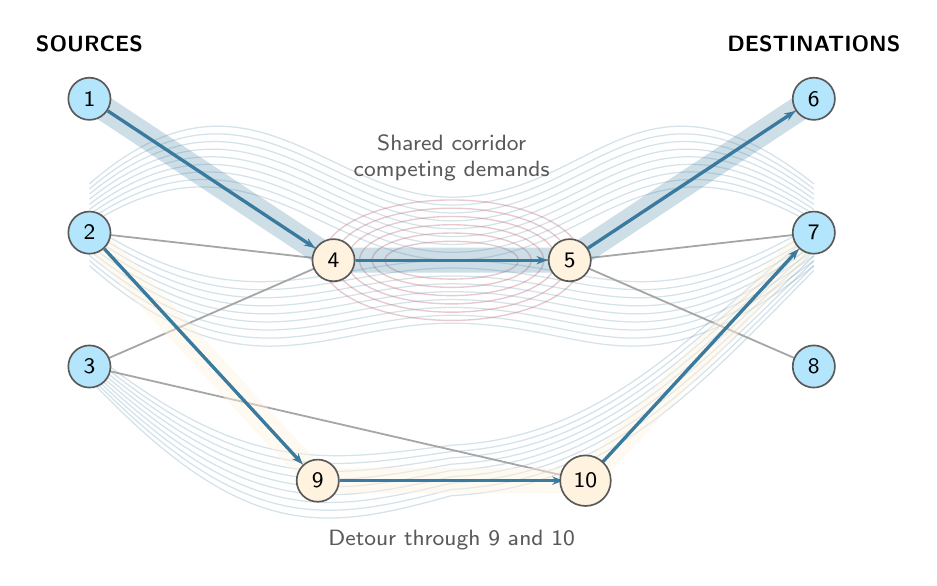
\begin{tikzpicture}[
 x=1cm,y=1cm,
 every node/.style={font=\sffamily\footnotesize,inner sep=3pt},
 >={Stealth[length=4pt,width=3pt]},
 device/.style={circle,draw=black!65,fill=white,minimum size=15pt,line width=.6pt},
 physical/.style={draw=black!35,line width=.65pt},
 annotation/.style={text=black!65,align=center,font=\sffamily\footnotesize}
]
% The field-like contours stay behind the physical network.
\begin{scope}[on background layer]
 \foreach \k in {0,...,8} {
  \draw[fieldblue,opacity=.22,line width=.45pt]
    (0,{2.9+.065*\k})
    .. controls (2,{4.2+.12*\k}) and (3,{2.45+.10*\k}) .. (4.6,{2.45+.10*\k})
    .. controls (6.4,{2.45+.10*\k}) and (7,{4.2+.12*\k}) .. (9.2,{2.9+.065*\k});
  \draw[fieldblue,opacity=.22,line width=.45pt]
    (0,{2.9-.065*\k})
    .. controls (2,{1.6-.12*\k}) and (3,{2.45-.10*\k}) .. (4.6,{2.45-.10*\k})
    .. controls (6.4,{2.45-.10*\k}) and (7,{1.6-.12*\k}) .. (9.2,{2.9-.065*\k});
  \draw[fieldblue,opacity=.22,line width=.45pt]
    (0,{1.3-.045*\k})
    .. controls (2,{-.3-.11*\k}) and (3,{-.1-.11*\k}) .. (4.6,{.1-.08*\k})
    .. controls (6.6,{.2-.08*\k}) and (7.7,{1.6-.10*\k}) .. (9.2,{2.8-.06*\k});
 }
 % Localized contention is conceptual, not a sampled pressure heat map.
 \foreach \k in {0,...,5} {
  \draw[fieldcoral,opacity=.32,line width=.5pt]
   (4.6,2.45) ellipse ({.85+.16*\k} and {.24+.105*\k});
 }
\end{scope}
\coordinate (n1) at (0,4.5);
\coordinate (n2) at (0,2.8);
\coordinate (n3) at (0,1.1);
\coordinate (n4) at (3.1,2.45);
\coordinate (n5) at (6.1,2.45);
\coordinate (n6) at (9.2,4.5);
\coordinate (n7) at (9.2,2.8);
\coordinate (n8) at (9.2,1.1);
\coordinate (n9) at (2.9,-.35);
\coordinate (n10) at (6.3,-.35);
% All eleven links from the fixture, with no invented geometric neighbors.
\foreach \a/\b in {1/4,2/4,3/4,4/5,5/6,5/7,5/8,2/9,9/10,10/7,3/10} {
 \draw[physical] (n\a) -- (n\b);
}
% Broad translucent bands distinguish route support from the contour metaphor.
\draw[fieldblue,opacity=.25,line width=9pt,line cap=round,line join=round]
 (n1) -- (n4) -- (n5) -- (n6);
\draw[fieldamber,opacity=.45,line width=9pt,line cap=round,line join=round]
 (n2) -- (n9) -- (n10) -- (n7);
\foreach \a/\b in {1/4,4/5,5/6} {
 \draw[fieldblue,line width=1.2pt,->,shorten <=8pt,shorten >=8pt] (n\a) -- (n\b);
}
\foreach \a/\b in {2/9,9/10,10/7} {
 \draw[fieldblue,line width=1.2pt,->,shorten <=8pt,shorten >=8pt] (n\a) -- (n\b);
}
\foreach \n in {1,2,3,6,7,8} {\node[device,fill=nodeblue] at (n\n) {\n};}
\foreach \n in {4,5,9,10} {\node[device,fill=nodeamber] at (n\n) {\n};}
\node[font=\sffamily\bfseries\footnotesize] at (0,5.2) {SOURCES};
\node[font=\sffamily\bfseries\footnotesize] at (9.2,5.2) {DESTINATIONS};
\node[annotation] at (4.6,3.75) {Shared corridor\\competing demands};
\node[annotation] at (4.6,-1.1) {Detour through 9 and 10};
\end{tikzpicture}
